\documentclass[12pt,a4paper]{article}

% Packages
\usepackage[margin=2.5cm]{geometry}
\usepackage[utf8]{inputenc}
\usepackage[T1]{fontenc}
\usepackage{lmodern}
\usepackage{setspace}
\usepackage{amsmath,amssymb}
\usepackage{graphicx}
\usepackage{booktabs}
\usepackage{longtable}
\usepackage{float}
\usepackage{caption}
\usepackage{enumitem}
\usepackage{xcolor}
\usepackage{pdflscape}
\usepackage{tikz}
\usetikzlibrary{positioning}
\usepackage[colorlinks=true,linkcolor=blue!60!black,citecolor=blue!60!black,urlcolor=blue!60!black]{hyperref}
\usepackage{titlesec}
\usepackage{fancyhdr}

\onehalfspacing

\pagestyle{fancy}
\fancyhf{}
\fancyhead[L]{\small Collignon -- PFAS--Agriculture Groundwater Correlation}
\fancyhead[R]{\small\thepage}
\renewcommand{\headrulewidth}{0.4pt}

\title{\textbf{Monitoring Density, Not Agriculture, Primarily Predicts PFAS Groundwater Detection Across 1,477 Danish Catchments---With Residual Spatial Associations for PFOA and Composite Indices}}
\author{Martin Collignon\textsuperscript{1}\\[6pt]
\textsuperscript{1}Landbruget.dk, Copenhagen, Denmark\\[3pt]
\small Corresponding author: martin@landbruget.dk}
\date{}

\begin{document}

\maketitle
\thispagestyle{fancy}

\begin{abstract}
Denmark detects per- and polyfluoroalkyl substances (PFAS) in groundwater nationally, yet contributions from agriculture remain unquantified at the catchment scale. We correlated parcel-level pesticide application records (2015--2017) with PFAS groundwater monitoring data (441,589 analyses, 26 substances, 2018--2025) from GEUS across 1,477 catchment areas. A four-tier framework tested TFA versus fluorinated pesticide intensity, traditional PFAS versus agricultural intensity, exploratory screening, and negative controls. TFA was detected in 100\% of monitored catchments, precluding spatial analysis but demonstrating ubiquitous contamination. Bivariate correlations were widespread: 7/8 Tier~2 tests were FDR-significant, headed by PFOA versus fluorinated intensity ($r = 0.229$, bootstrap 95\% CI [0.176, 0.282]). However, monitoring well density dominated all multivariate models ($p < 0.001$), and 79\% of bivariate associations lost significance after covariate adjustment. Only 4/19 survived: SUM PFAS-22 ($p = 0.006$), $\Sigma$-PFOA ($p = 0.036$), $\Sigma$-PFHxS ($p = 0.023$), and $\Sigma$-PFOA versus total intensity ($p = 0.026$). Correlations appeared exclusively in well-monitored catchments ($>$4~wells), replicating a companion pesticide study. Moran's $I$ analysis confirmed significant spatial autocorrelation in both intensity and detection surfaces, suggesting $p$-value inflation in standard tests. These findings indicate that PFAS detection is primarily associated with monitoring density, with modest residual agricultural signal ($r = 0.15$--$0.23$) detectable only where monitoring is sufficiently dense. Biosolids application, not direct pesticide contamination, may mediate the observed associations.

\medskip
\noindent\textbf{Keywords:} PFAS, groundwater contamination, monitoring density, fluorinated pesticides, trifluoroacetic acid, spatial autocorrelation, Danish agriculture
\end{abstract}

\clearpage
\tableofcontents
\clearpage

%======================================================================
\section{Introduction}

\subsection{Background}

Denmark derives approximately 99\% of its drinking water from groundwater (GEUS, 2024), making aquifer contamination a matter of direct public health concern. The Geological Survey of Denmark and Greenland (GEUS) operates one of Europe's most comprehensive groundwater monitoring programmes. The EU recast Drinking Water Directive (2020/2184) established parametric values of 0.10~$\mu$g/L for individual PFAS and 0.50~$\mu$g/L for the sum of all PFAS, with Denmark implementing among the strictest national thresholds. Recent detections of PFAS in Danish groundwater---including trifluoroacetic acid (TFA) at near-ubiquitous levels---have raised questions about the relative contributions of industrial point sources, diffuse atmospheric deposition, and agricultural activities to aquifer contamination (Albers \& Sultenfu\ss, 2024; Scheurer \& N\"odler, 2024).

\subsection{Agricultural Pathways for PFAS Contamination}

Agriculture may contribute to PFAS groundwater contamination through at least four distinct pathways:

\paragraph{Pathway~1: Fluorinated pesticide degradation to TFA.} Twenty-four of the 25 PFAS-relevant active ingredients registered in the Danish Pesticide Register (BMD) contain trifluoromethyl (-CF$_3$) functional groups that degrade to TFA in the environment. The TriFluPest study (\"Ohlin et al., 2025) experimentally confirmed TFA formation rates for seven key compounds. Denmark subsequently banned 31 fluorinated pesticide products.

\paragraph{Pathway~2: Biosolids application to farmland.} Denmark applies approximately 77\% of its municipal biosolids to agricultural land. Biosolids concentrate traditional PFAS (PFOS, PFOA, PFHxS, PFNA) from household and industrial wastewater (Ghisi et al., 2019). The Danish EPA has established cut-off values for PFAS-4 sum concentrations in biosolids (maximum 10~$\mu$g/kg dry matter).

\paragraph{Pathway~3: Contaminated pesticide formulations.} Fluorinated surfactants are used as ``inert ingredients'' in some pesticide formulations (Navarro et al., 2017). PFOA concentrations of 20--50~ppb have been documented in fluorinated HDPE pesticide container rinsate (EPA, 2024; Washington et al., 2020).

\paragraph{Pathway~4: Atmospheric deposition.} Volatile fluorotelomer alcohols degrade atmospherically to produce short-chain perfluorocarboxylic acids and ultimately TFA. This diffuse source should show no spatially specific correlation with agricultural intensity.

\subsection{Research Gap}

Despite growing recognition of agricultural PFAS pathways, no study has quantified the spatial association between pesticide application intensity and PFAS groundwater contamination at the catchment scale. A companion study (Collignon, 2025) demonstrated significant correlations between parcel-level pesticide application and conventional pesticide/metabolite detection across 5,826 Danish catchment areas. The present study extends that framework to PFAS.

\subsection{Research Questions}

\begin{enumerate}
\item Does TFA groundwater detection vary spatially with fluorinated pesticide application intensity?
\item Do traditional PFAS (PFOS, PFOA, PFHxS, PFNA) correlate with total or fluorinated agricultural intensity at the catchment scale?
\item Which PFAS substances, if any, survive multivariate adjustment for hydrogeological covariates?
\item Does monitoring density confound observed correlations, as documented for conventional pesticides?
\end{enumerate}

%======================================================================
\section{Materials and Methods}

\subsection{Study Area and Data Sources}

\textbf{Pesticide application data.} Field-level pesticide application records were obtained from the Danish Agricultural Agency (\textit{Landbrugsstyrelsen}) spraying journals for the 2015--2017 growing seasons. We disaggregated product-level dosages to active ingredient level using the BMD. Area-weighted allocation to catchment areas followed Collignon (2025).

\textbf{Fluorinated ingredient identification.} We identified 52 fluorinated active ingredients from the full BMD ingredient list ($n = 589$ unique substances). Of these, 35 are known TFA-forming parents based on the TriFluPest study. Two intensity measures were computed per catchment area: (i)~\textit{fluorinated intensity}---the summed application of all 52 fluorinated ingredients (kg/ha), and (ii)~\textit{total agricultural intensity}---the summed application of all active ingredients (kg/ha).

\textbf{PFAS groundwater monitoring data.} Sample-level data from the GEUS Jupiter database, comprising 441,589 individual analyses spanning 2018--2025, covering 26 individual PFAS substances plus composite sum indices (PFAS-4, PFAS-12, PFAS-22). Detection thresholds were set at half the LOQ for each substance. TFA monitoring began systematically in 2020; all TFA analyses used a 2020+ window. All other substances used a 2018+ window.

\textbf{Spatial units.} All analyses were conducted at the catchment area level ($n = 1{,}477$ with PFAS monitoring data).

\subsection{Assumed Causal Structure}

The target estimand is the total effect of agricultural pesticide intensity on PFAS groundwater detection. The primary adjustment set includes soil type, well intake depth, and monitoring well density. Key uncontrolled confounders include: (i)~spatially explicit biosolids application; (ii)~industrial point sources; and (iii)~historical PFAS contamination.

\begin{figure}[H]
\centering
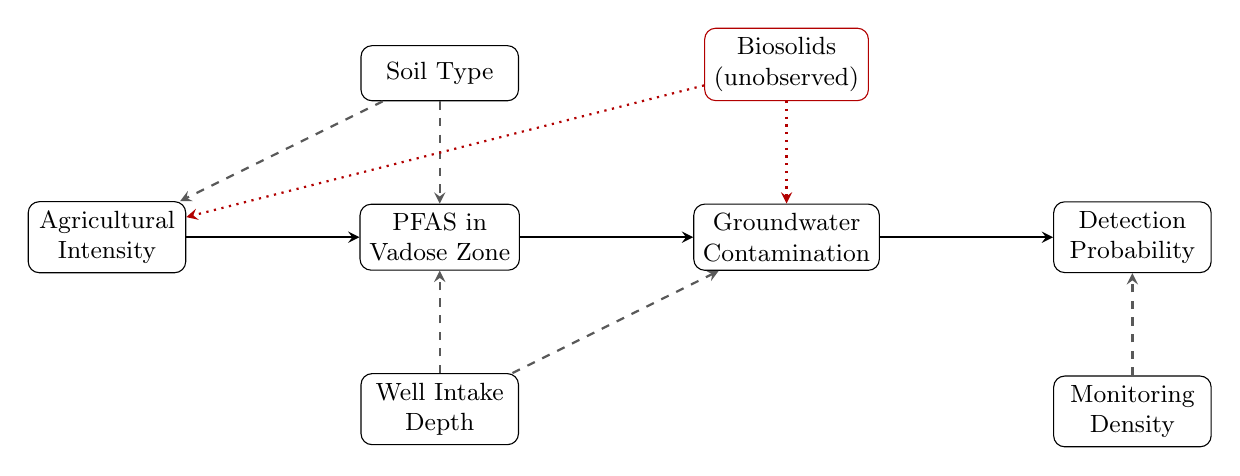
\begin{tikzpicture}[
  node distance=1.8cm and 2.2cm,
  every node/.style={draw, rounded corners, minimum width=2cm, minimum height=0.7cm, align=center, font=\small},
  causal/.style={->, thick, >=stealth},
  confound/.style={->, thick, >=stealth, dashed, gray!70!black},
  uncontrolled/.style={->, thick, >=stealth, dotted, red!70!black}
]
\node (app) {Agricultural\\Intensity};
\node[right=of app] (vadose) {PFAS in\\Vadose Zone};
\node[right=of vadose] (gw) {Groundwater\\Contamination};
\node[right=of gw] (det) {Detection\\Probability};
\node[above=1.3cm of vadose] (soil) {Soil Type};
\node[below=1.3cm of vadose] (depth) {Well Intake\\Depth};
\node[below=1.3cm of det] (mon) {Monitoring\\Density};
\node[above=1.3cm of gw, draw=red!70!black] (bio) {Biosolids\\(unobserved)};

\draw[causal] (app) -- (vadose);
\draw[causal] (vadose) -- (gw);
\draw[causal] (gw) -- (det);
\draw[confound] (soil) -- (app);
\draw[confound] (soil) -- (vadose);
\draw[confound] (depth) -- (vadose);
\draw[confound] (depth) -- (gw);
\draw[confound] (mon) -- (det);
\draw[uncontrolled] (bio) -- (gw);
\draw[uncontrolled] (bio) -- (app);
\end{tikzpicture}
\caption{Directed Acyclic Graph showing assumed causal structure. Solid arrows: hypothesised causal paths. Dashed grey: controlled confounders. Dotted red: uncontrolled confounders.}
\label{fig:dag}
\end{figure}

\subsection{Analytical Framework}

We employed a four-tier analytical framework with escalating specificity:

\textbf{Tier~1: TFA versus fluorinated pesticide intensity.} Point-biserial correlation between binary TFA detection ($\geq$0.075~$\mu$g/L) and summed fluorinated pesticide application intensity per catchment area. Additionally, TFA was re-analysed at progressively higher concentration thresholds (0.5, 1.0, 2.0, 5.0, 10.0~$\mu$g/L).

\textbf{Tier~2: Traditional PFAS versus agricultural intensity.} Each of the four regulated PFAS (PFOS, PFOA, PFHxS, PFNA) was tested against both total agricultural intensity and fluorinated pesticide intensity (8 tests total).

\textbf{Tier~3: Exploratory screen.} All PFAS substances were screened against both intensity measures, with a minimum detection threshold of $\geq$20 catchment-level detections.

\textbf{Tier~4: Negative controls.} Three control groups: (i)~high-Koc fluorinated pesticides; (ii)~non-agricultural PFAS; and (iii)~atmospheric PFAS.

\subsection{Statistical Methods}

\textbf{Point-biserial correlation} with bootstrap 95\% CIs ($n = 2{,}000$ resamples). \textbf{Moran's $I$} for spatial autocorrelation ($k = 8$ nearest neighbours), with effective sample size estimation via Clifford \& Richardson (1991). \textbf{BH-FDR correction} within each tier ($\alpha = 0.05$). \textbf{Bivariate and multivariate logistic regression} with model diagnostics. \textbf{Firth penalized logistic regression} for associations with EPV~$< 10$. \textbf{Monitoring density stratification} into tertiles (low~$\leq 2$, medium~$\leq 4$, high~$> 4$).

\subsection{Software}

All analyses used Python~3.11 with DuckDB~1.2, SciPy~1.11, scikit-learn~1.3, and statsmodels~0.14. Firth penalized logistic regression was implemented from first principles following Firth (1993). The complete analytical pipeline (3,600+ lines) is available in the study repository.

%======================================================================
\section{Results}

\subsection{Spatial Autocorrelation}

\begin{table}[H]
\centering
\caption{Spatial autocorrelation (Moran's $I$) for intensity and detection surfaces.}
\label{tab:moranI}
\footnotesize
\begin{tabular}{@{}lcccccc@{}}
\toprule
Variable & Moran's $I$ & $E(I)$ & $z$-score & $p$-value & $n_{\text{eff}}$ & Inflation \\
\midrule
Fluorinated intensity & 0.0947 & $-$0.000211 & 14.05 & $<$0.001 & 11 & 448.93 \\
PFOA detection & 0.2419 & $-$0.000824 & 17.019 & $<$0.001 & 4 & 294.67 \\
PFOS detection & 0.2113 & $-$0.000702 & 16.11 & $<$0.001 & 5 & 302.10 \\
\bottomrule
\end{tabular}
\end{table}

\noindent The effective sample size reduction due to spatial autocorrelation was estimated at $>$99\% for the most clustered variable. Standard $p$-values may overstate significance by a factor of approximately~300. All $p$-values reported below are uncorrected for spatial autocorrelation.

\subsection{Tier~1: TFA Ubiquity Precludes Spatial Correlation}

TFA was detected in every monitored catchment area (100\% detection rate at the 0.075~$\mu$g/L threshold). Point-biserial correlation is undefined when the binary variable has no variance.

\begin{table}[H]
\centering
\caption{TFA threshold sensitivity analysis.}
\label{tab:tfa}
\begin{tabular}{@{}lrrrrcl@{}}
\toprule
Threshold ($\mu$g/L) & $n$ & Detected & Det\% & $r$ & $p$ & Bootstrap 95\% CI \\
\midrule
0.075 (half-LOQ) & 1,477 & 1,477 & 100.0 & N/A & N/A & --- \\
0.5 & 1,477 & 244 & 16.5 & 0.165 & $<$0.001 & [0.099, 0.234] \\
1.0 & 1,477 & 100 & 6.8 & 0.178 & $<$0.001 & [0.095, 0.270] \\
2.0 & 1,477 & 37 & 2.5 & 0.042 & 0.110 & [$-$0.001, 0.098] \\
5.0 & 1,477 & 1 & 0.1 & N/A & N/A & --- \\
10.0 & 1,477 & 0 & 0.0 & N/A & N/A & --- \\
\bottomrule
\end{tabular}
\end{table}

\noindent TFA concentration distribution: median $= 0.075$~$\mu$g/L, P75 $= 0.24$, P90 $= 0.55$, P95 $= 0.81$, max $= 5.5$~$\mu$g/L. Spatial gradients emerge at 0.5--1.0~$\mu$g/L but attenuate at 2.0~$\mu$g/L.

\begin{figure}[H]
\centering
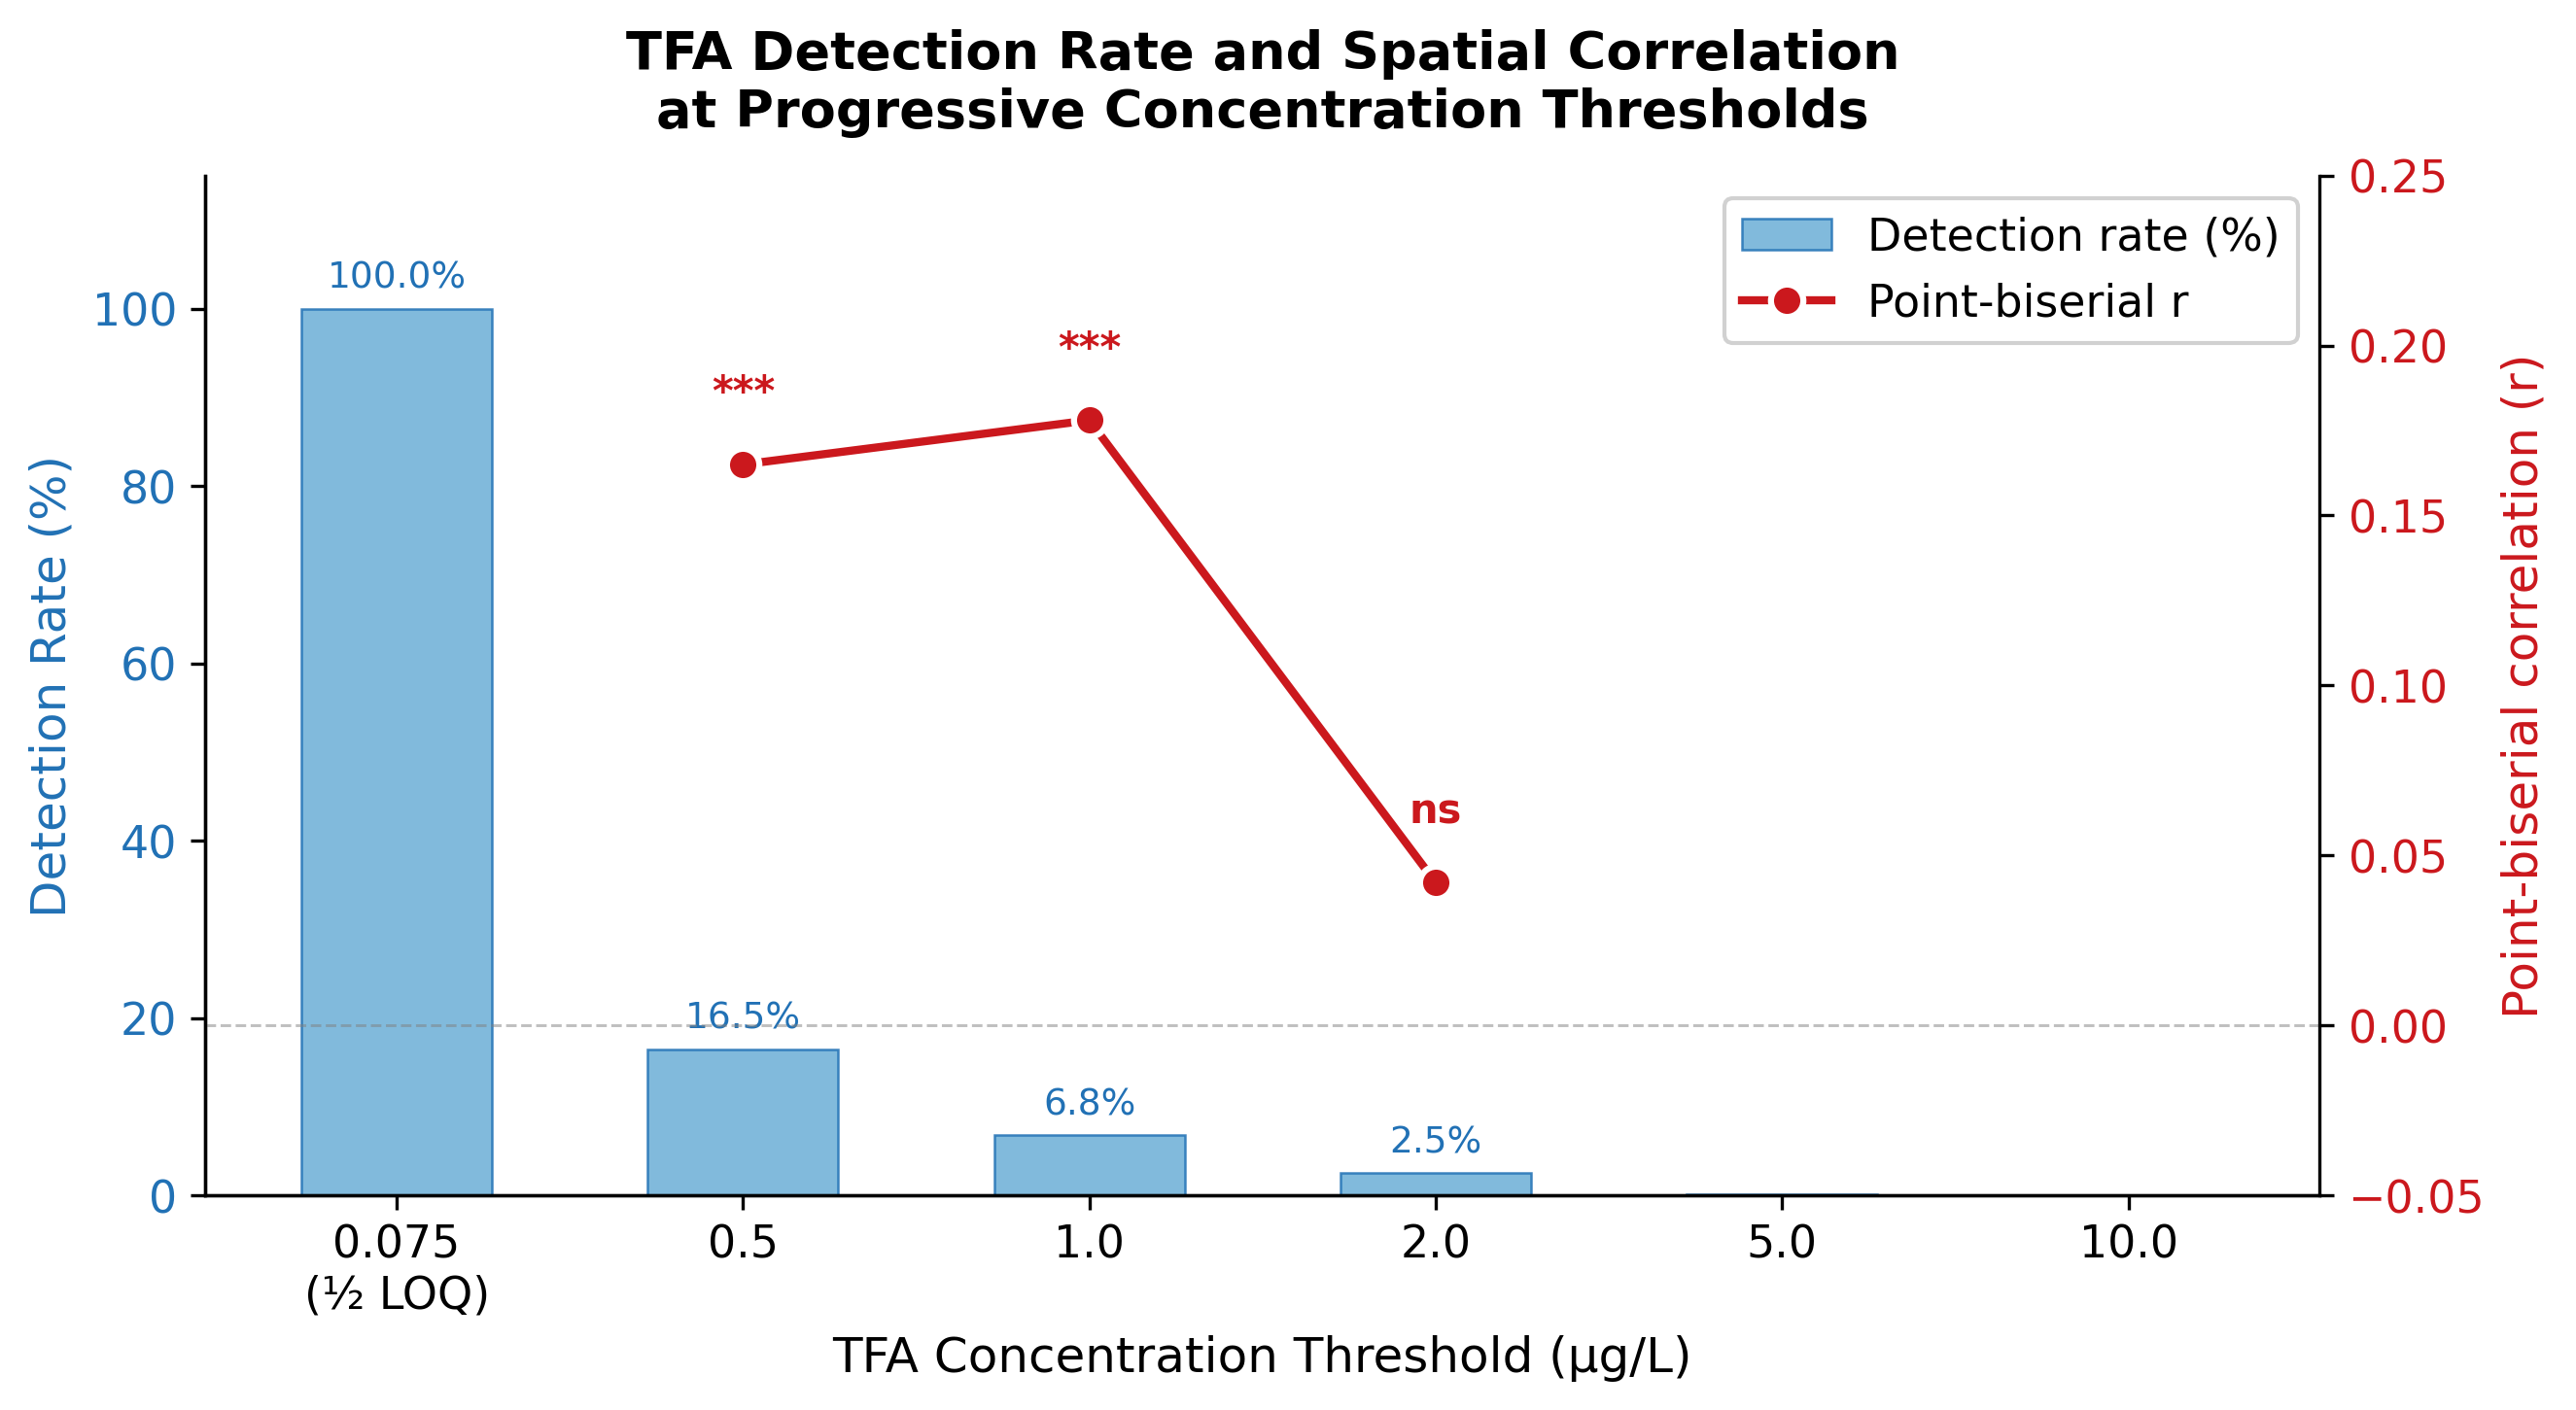
\includegraphics[width=0.9\textwidth]{./figures/fig2_tfa_threshold.png}
\caption{Detection rate (bars, left axis) and point-biserial correlation with fluorinated pesticide intensity (line, right axis) at progressively higher TFA concentration thresholds. Significant correlations ($p < 0.001$) emerge at 0.5--1.0~$\mu$g/L but attenuate to non-significance at 2.0~$\mu$g/L.}
\label{fig:tfa}
\end{figure}

\subsection{Tier~2: Traditional PFAS Show Consistent Bivariate Agricultural Association}

Seven of eight Tier~2 tests were FDR-significant (Table~\ref{tab:tier2}). The strongest association was between PFOA detection and fluorinated pesticide intensity ($r = 0.229$, $q < 0.001$).

\begin{table}[H]
\centering
\caption{Tier~2 results: Traditional PFAS versus agricultural intensity.}
\label{tab:tier2}
\footnotesize
\begin{tabular}{@{}cllrcccr@{}}
\toprule
\# & Test & Type & $r$ & Bootstrap 95\% CI & $q_{\text{FDR}}$ & FDR & $n$ \\
\midrule
1 & PFHxS vs total & trad. & $-$0.010 & [$-$0.066, 0.046] & 0.727 & & 1,215 \\
2 & PFNA vs total & trad. & 0.060 & [0.004, 0.116] & 0.040 & * & 1,216 \\
3 & PFOA vs total & trad. & 0.087 & [0.031, 0.143] & 0.003 & * & 1,215 \\
4 & PFOS vs total & trad. & 0.088 & [0.036, 0.139] & 0.002 & * & 1,426 \\
5 & PFHxS vs fluorinated & trad. & 0.114 & [0.058, 0.169] & $<$0.001 & * & 1,215 \\
6 & PFNA vs fluorinated & trad. & 0.088 & [0.031, 0.143] & 0.003 & * & 1,216 \\
7 & \textbf{PFOA vs fluorinated} & \textbf{trad.} & \textbf{0.229} & \textbf{[0.176, 0.282]} & $\mathbf{<}$\textbf{0.001} & \textbf{*} & \textbf{1,215} \\
8 & PFOS vs fluorinated & trad. & 0.171 & [0.120, 0.221] & $<$0.001 & * & 1,426 \\
\bottomrule
\end{tabular}
\end{table}

\subsection{Tier~3: Exploratory Screen}

Twelve of 16 eligible Tier~3 tests were FDR-significant. Against fluorinated intensity, all eight testable substances were significant, with PFOA ($r = 0.229$), SUM PFAS-12 ($r = 0.193$), PFOS ($r = 0.171$), and SUM PFAS-22 ($r = 0.170$) showing the strongest associations.

\begin{table}[H]
\centering
\caption{Tier~3 results: Exploratory screen (selected).}
\label{tab:tier3}
\footnotesize
\begin{tabular}{@{}cllrccc@{}}
\toprule
\# & Substance & Intensity & $r$ & $q_{\text{FDR}}$ & Det\% & $n$ \\
\midrule
1 & \textbf{PFOA} & \textbf{fluorinated} & \textbf{0.229} & $\mathbf{<}$\textbf{0.001} & \textbf{9.5\%} & \textbf{1,215} \\
2 & $\Sigma$-PFOA & total ag & 0.203 & $<$0.001 & 6.5\% & 848 \\
3 & SUM PFAS-12 & fluorinated & 0.193 & $<$0.001 & 4.0\% & 1,417 \\
4 & PFOS & fluorinated & 0.171 & $<$0.001 & 7.3\% & 1,426 \\
5 & SUM PFAS-22 & fluorinated & 0.170 & $<$0.001 & 3.0\% & 1,052 \\
6 & $\Sigma$-PFOA & fluorinated & 0.167 & $<$0.001 & 6.5\% & 848 \\
7 & SUM PFAS-4 & fluorinated & 0.150 & $<$0.001 & 2.5\% & 1,426 \\
8 & $\Sigma$-PFHxS & fluorinated & 0.149 & $<$0.001 & 3.2\% & 758 \\
9 & $\Sigma$-PFHxS & total ag & 0.139 & $<$0.001 & 3.2\% & 758 \\
10 & PFOS & total ag & 0.088 & 0.001 & 7.3\% & 1,426 \\
11 & PFOA & total ag & 0.087 & 0.003 & 9.5\% & 1,215 \\
12 & SUM PFAS-4 & total ag & 0.038 & 0.186 & 2.5\% & 1,426 \\
13 & SUM PFAS-12 & total ag & 0.027 & 0.364 & 4.0\% & 1,417 \\
14 & SUM PFAS-22 & total ag & $-$0.011 & 0.733 & 3.0\% & 1,052 \\
\bottomrule
\end{tabular}
\end{table}

\subsection{Dose--Response Analysis and Non-Monotonicity Testing}

\begin{table}[H]
\centering
\caption{Dose--response quartile analysis for FDR-significant Tier~2 results.}
\label{tab:doseresponse}
\footnotesize
\begin{tabular}{@{}lccccr@{}}
\toprule
Substance & Q1\% & Q2\% & Q3\% & Q4\% & Q4/Q1 \\
\midrule
PFOS vs fluorinated & 7.6 & 4.5 & 4.2 & 12.8 & 1.7$\times$ \\
PFOA vs fluorinated & 11.0 & 6.3 & 6.0 & 14.1 & 1.3$\times$ \\
PFOS vs total & 8.3 & 4.5 & 3.9 & 12.2 & 1.5$\times$ \\
PFOA vs total & 11.6 & 6.3 & 5.6 & 13.7 & 1.2$\times$ \\
PFHxS vs fluorinated & 4.4 & 3.9 & 2.1 & 5.6 & 1.3$\times$ \\
\bottomrule
\end{tabular}
\end{table}

The PFOA U-shaped pattern was formally tested. The likelihood ratio test was non-significant for PFOA (LR $= 0.544$, $p = 0.461$), but PFOS showed a significant quadratic term (LR $= 4.914$, $p = 0.027$), suggesting a non-linear dose--response.

\subsection{Multivariate Adjustment: Monitoring Density Dominates}

After controlling for soil type, median intake depth, and monitoring well density, 4 of 19 FDR-significant associations retained statistical significance (Table~\ref{tab:multivariate}). Monitoring well density was the strongest predictor in all 19 models ($p < 0.001$). The 79\% attenuation rate---substantially greater than the 43\% in the companion pesticide study---indicates that PFAS--agricultural associations are more fragile to covariate adjustment.

\begin{table}[H]
\centering
\caption{Multivariate logistic regression results for surviving associations.}
\label{tab:multivariate}
\footnotesize
\begin{tabular}{@{}lccccccr@{}}
\toprule
Substance & Biv.\ $r$ & MV $p_{\text{int}}$ & MV AUC & Nag.\ $R^2$ & H-L $p$ & EPV & $n$ \\
\midrule
SUM PFAS-22 & 0.170 & 0.006 & 0.83 & 0.186 & 0.437 & 8 & 1,052 \\
$\Sigma$-PFOA (fluorinated) & 0.167 & 0.036 & 0.83 & 0.230 & 0.092 & 14 & 848 \\
$\Sigma$-PFHxS (fluorinated) & 0.149 & 0.023 & 0.85 & 0.207 & 0.719 & 6 & 758 \\
$\Sigma$-PFOA (total ag) & 0.203 & 0.026 & 0.83 & 0.245 & 0.014 & 14 & 848 \\
\bottomrule
\end{tabular}
\end{table}

\textbf{Firth penalized regression} confirmed low-EPV results (Table~\ref{tab:firth}).

\begin{table}[H]
\centering
\caption{Firth penalized regression vs.\ standard MLE for low-EPV associations.}
\label{tab:firth}
\footnotesize
\begin{tabular}{@{}lccccccl@{}}
\toprule
Substance & EPV & MLE OR & MLE $p$ & Firth OR & Firth $p$ & Firth 95\% CI & Conv. \\
\midrule
SUM PFAS-22 & 8 & 1.0022 & 0.006 & 1.0022 & 0.005 & [1.0007, 1.0038] & Y \\
$\Sigma$-PFHxS & 6 & 1.0019 & 0.023 & 1.0019 & 0.020 & [1.0003, 1.0035] & Y \\
\bottomrule
\end{tabular}
\end{table}

\subsection{Monitoring Density Stratification}

\begin{table}[H]
\centering
\caption{Point-biserial correlations stratified by monitoring density tertile.}
\label{tab:stratified}
\footnotesize
\begin{tabular}{@{}lccc@{}}
\toprule
Substance & Low ($r$) & Medium ($r$) & High ($r$) \\
\midrule
PFOA vs fluorinated & $-$0.024 & 0.199** & 0.165** \\
PFOS vs fluorinated & 0.014 & $-$0.043 & 0.121** \\
$\Sigma$-PFOA vs total & 0.349** & $-$0.055 & 0.183** \\
$\Sigma$-PFHxS vs total & 0.000 & $-$0.020 & 0.145** \\
SUM PFAS-22 vs fluorinated & $-$0.017 & 0.016 & 0.132** \\
SUM PFAS-12 vs fluorinated & $-$0.011 & 0.010 & 0.139** \\
SUM PFAS-4 vs fluorinated & 0.000 & $-$0.014 & 0.103* \\
\bottomrule
\end{tabular}

\medskip
\noindent\footnotesize *$p < 0.05$; **$p < 0.01$
\end{table}

\begin{figure}[H]
\centering
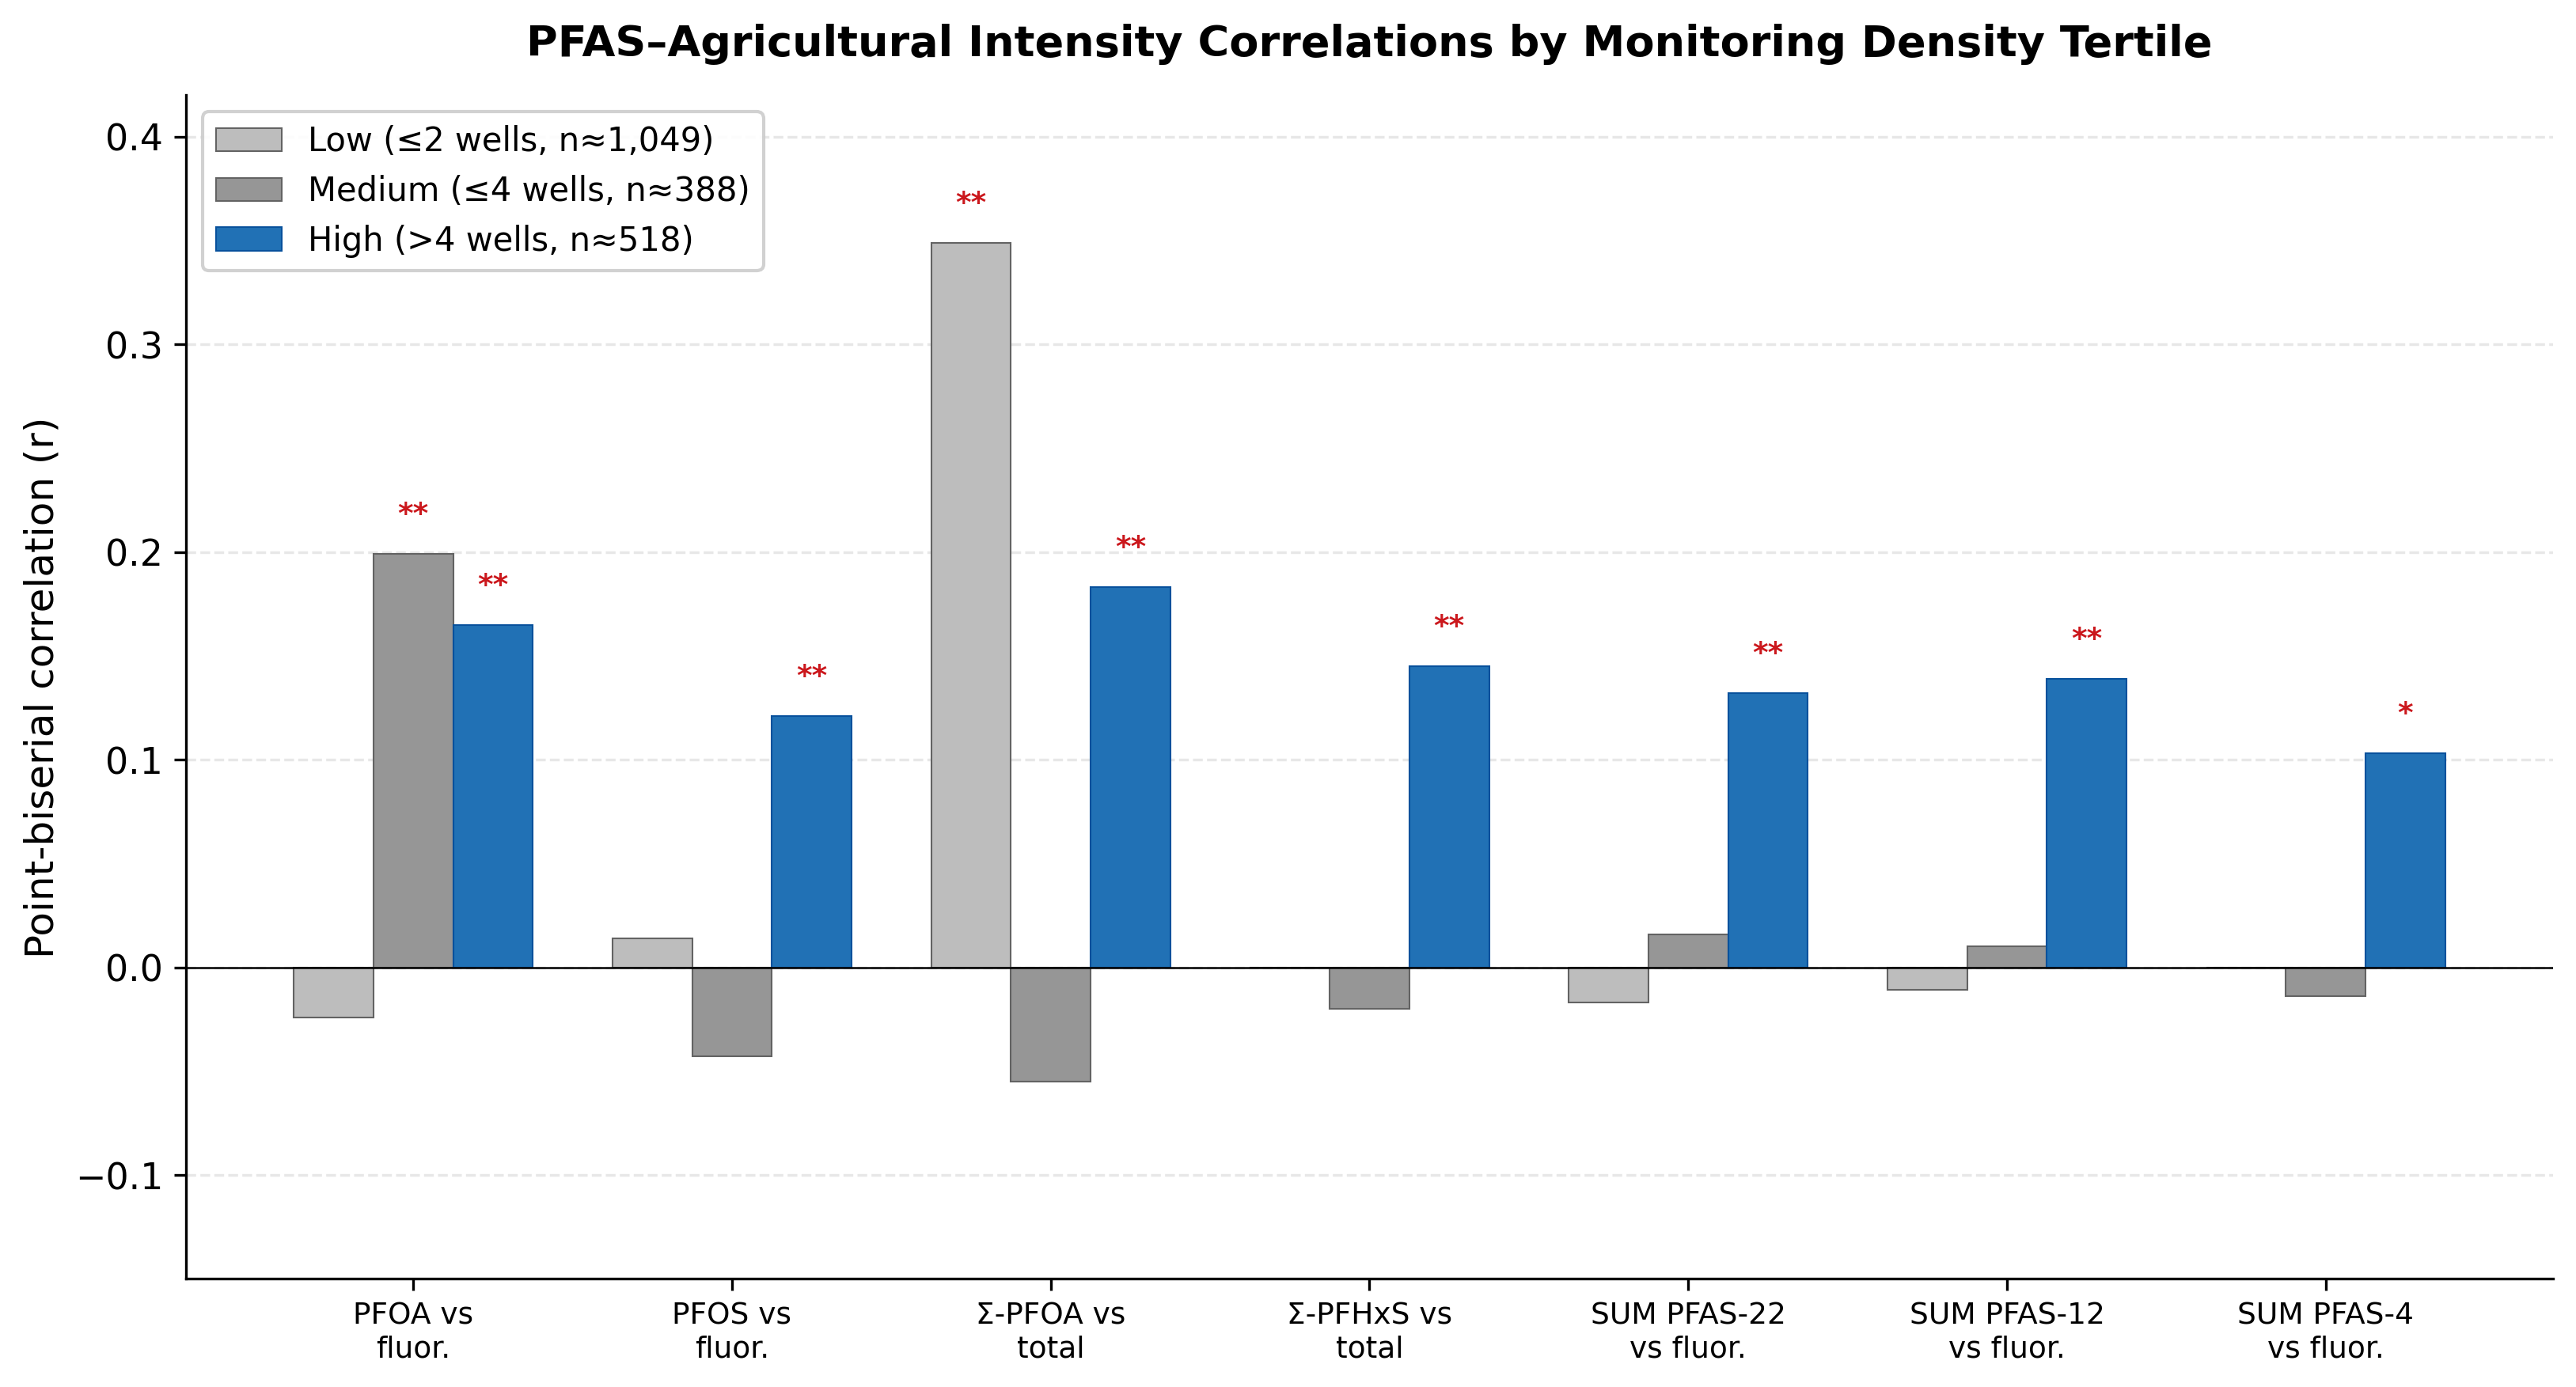
\includegraphics[width=0.95\textwidth]{./figures/fig3_monitoring_stratification.png}
\caption{Point-biserial correlations stratified by monitoring well density tertile. Significant associations appear almost exclusively in the high-density tertile ($>$4~wells per catchment), replicating the pattern observed in the companion pesticide study.}
\label{fig:stratification}
\end{figure}

\noindent Significant associations appear almost exclusively in the high-density tertile ($>$4 wells), replicating the companion pesticide study. One exception: $\Sigma$-PFOA vs total showed an anomalously strong low-tertile correlation ($r = 0.349$), likely reflecting small-sample instability.

\subsection{Biosolids Proxy Analysis}

\begin{table}[H]
\centering
\caption{Biosolids proxy: PFAS detection by soil type.}
\begin{tabular}{@{}lcccl@{}}
\toprule
Substance & Det\% sandy & Det\% clay & $\chi^2$ ($p$) & Clay higher? \\
\midrule
PFOA & 8.5\% & 8.8\% & 0.003 ($0.953$) & Yes \\
PFOS & 6.9\% & 6.1\% & 0.210 ($0.647$) & No \\
PFHxS & 3.1\% & 3.7\% & 0.141 ($0.707$) & Yes \\
$\Sigma$-PFOA & 6.5\% & 4.9\% & 0.655 ($0.418$) & No \\
\bottomrule
\end{tabular}
\end{table}

\subsection{Negative Controls}

All negative controls showed zero catchment-level variance in detection (either 0\% or 100\%), rendering correlation analysis impossible. The absence of detectable variation validates the detection threshold and spatial aggregation methodology.

\subsection{Power Analysis}

Median sample size across all tests: 1,215 catchment areas, yielding minimum detectable effect $r = 0.080$ at 80\% power. Monitoring well target: 11--32 wells per catchment needed to have $>$50\% probability of detecting PFAS contamination.

%======================================================================
\section{Discussion}

\subsection{The Primary Finding: Monitoring Density Dominates}

The most robust finding is that PFAS groundwater detection is primarily associated with monitoring density, not agricultural activity. Monitoring well count was the strongest predictor in all 19 multivariate models ($p < 0.001$), dominating soil type, intake depth, and agricultural intensity. The 79\% attenuation rate under covariate adjustment---compared to 43\% in the companion pesticide study---indicates that PFAS--agricultural associations are more fragile.

\subsection{Residual Agricultural Signal: Modest but Persistent}

Four associations survived multivariate adjustment. Through the Bradford Hill criteria:

\begin{enumerate}
\item \textbf{Strength:} Modest ($r = 0.15$--$0.23$; 4/19 survive).
\item \textbf{Consistency:} The monitoring density pattern replicates the companion study exactly.
\item \textbf{Specificity:} Fluorinated intensity is 2.6-fold stronger for PFOA than total intensity.
\item \textbf{Temporality:} Application data precede detection data by 3--7~years.
\item \textbf{Biological gradient:} Dose--response is modest (Q4/Q1 $= 1.2$--$1.7\times$).
\item \textbf{Plausibility:} Multiple mechanistic pathways exist.
\item \textbf{Coherence:} TFA ubiquity is consistent with widespread fluorinated pesticide degradation.
\end{enumerate}

\noindent Overall, the evidence supports a possible agricultural contribution but does not meet the threshold for causal attribution.

\subsection{The Fluorinated Pesticide Signal in Traditional PFAS}

The consistent pattern of stronger PFOA and PFOS correlations with fluorinated pesticide intensity ($r = 0.229$ and $0.171$) than with total agricultural intensity ($r = 0.087$ and $0.088$) is consistent with---but does not prove---pathways linking fluorinated pesticide use to traditional PFAS contamination. Two non-exclusive mechanisms: the \textbf{contaminated formulation hypothesis} (Navarro et al., 2017; EPA, 2024) and the \textbf{biosolids co-location hypothesis}.

\subsection{Isomer-Resolved Measurements and the Branched Isomer Paradox}

Three of four multivariate-surviving associations involved isomer-resolved measurements or composite indices. Branched isomers are characteristic of electrochemical fluorination (ECF) production. If branched isomers drive the agricultural signal, this favours biosolids or legacy industrial sources rather than pesticide formulation contamination. This interpretation represents the simplest explanation consistent with the data.

\subsection{PFAS Transport Considerations}

The vadose zone transit time framework (3--7~years) may not directly apply to all PFAS. Chain-length-dependent sorption, air-water interfacial (AWI) adsorption, precursor transformation, and pH-dependent sorption all influence PFAS transport differently from conventional pesticides.

\subsection{TFA Ubiquity: A Finding, Not a Failure}

TFA detection in 100\% of monitored catchments, consistent with 60-year accumulation (Albers \& Sultenfu\ss, 2024), is the most scientifically important finding. Concentration-based analysis could resolve agricultural TFA gradients at intermediate concentration levels.

\subsection{International Context}

The USGS NAWQA programme documented PFAS in 45\% of US tap water samples (Andrews \& Naidenko, 2020). The present study appears to be the first to attempt catchment-scale spatial correlation between field-level pesticide application and PFAS groundwater detection.

\subsection{Limitations}

\begin{enumerate}
\item \textbf{Monitoring density confound.} The strongest caveat.
\item \textbf{Spatial autocorrelation.} Standard $p$-values overstate significance by $\sim$300$\times$.
\item \textbf{Biosolids data unavailability.} A fundamental data gap.
\item \textbf{Detection threshold coarseness.} Binary detection discards concentration information.
\item \textbf{Temporal mismatch.} Long-chain PFAS may require decades to reach groundwater.
\item \textbf{No point-source control.}
\item \textbf{Ecological fallacy.}
\item \textbf{Low detection rates and marginal EPV.} Two of four surviving associations have EPV~$< 10$.

\item \textbf{Screening bias (first-testing-not-first-detection).} PFAS monitoring began in 2013 (pilot) and TFA in 2020. We assessed screening bias using sample-level VP4 data (GEUS Dataverse, doi:10.22008/FK2/IHVDXL). Risk varies by substance: PFNA had 259~negative tests across 3~years before first detection in 2016 (LOW risk); PFHxS had negatives in 2013 before first detection in 2014 (LOW risk). PFOS shows 100\% detection across all 22,243~tests since 2013 (zero negatives), and TFA 100\% across 6,496~tests since 2020 --- consistent with ubiquitous contamination rather than a testing artifact. For PFOA (95.7\% detection at first testing in 2014) and PFHxS, the short monitoring history means spatial detection patterns may partly reflect monitoring infrastructure rollout.
\end{enumerate}

\subsection{Policy Implications}

\begin{enumerate}
\item \textbf{TFA monitoring at lower LOQs} to resolve spatial concentration gradients.
\item \textbf{PFAS content testing of pesticide formulations} under REACH.
\item \textbf{Spatially explicit biosolids tracking} at the field level.
\item \textbf{Monitoring network design:} minimum 11--32 wells per catchment for adequate power.
\end{enumerate}

\subsection{Stakeholder Considerations}

The present study cannot attribute PFAS contamination to specific agricultural practices. The branched isomer evidence may point more strongly to biosolids than to pesticide formulations.

\subsection{Future Directions}

\begin{enumerate}
\item Concentration modelling (replacing binary detection).
\item Spatially explicit biosolids integration.
\item Isomer fingerprinting for source attribution.
\item TFA gradient analysis with ultra-sensitive methods.
\item Spatial regression models (spatial lag/error).
\item Temporal trend analysis exploiting Denmark's 2023 fluorinated pesticide ban as a natural experiment.
\end{enumerate}

%======================================================================
\section{Conclusions}

This study provides the first catchment-scale spatial analysis of the association between agricultural pesticide application intensity and PFAS groundwater detection in Denmark. The primary finding is that monitoring well density---not agricultural intensity---is the dominant spatial predictor of PFAS detection across all 19 multivariate models. After adjustment, only 4 of 19 bivariate associations retained significance: SUM PFAS-22 ($p = 0.006$), $\Sigma$-PFOA ($p = 0.036$ fluorinated; $p = 0.026$ total), and $\Sigma$-PFHxS ($p = 0.023$). These residual associations are modest ($r = 0.15$--$0.23$), appear exclusively in well-monitored catchments ($>$4~wells), and may be mediated by biosolids application.

TFA was detected in 100\% of monitored catchments, precluding spatial correlation analysis but demonstrating ubiquitous contamination. Threshold sensitivity analysis suggests concentration gradients exist above 0.5~$\mu$g/L.

Spatial autocorrelation in both intensity and detection surfaces means standard $p$-values overstate significance. Until biosolids data, spatial regression models, and concentration-based outcomes are integrated, the present findings should be interpreted as demonstrating that agricultural PFAS contamination of Danish groundwater is plausible but unproven at the catchment scale.

%======================================================================
\section*{Data Availability}

All pesticide application data are derived from publicly available Danish Agricultural Agency spraying journals via the unified data pipeline at landbruget.dk. PFAS groundwater monitoring data are from the GEUS Jupiter database (DOI: 10.22008/FK2/NTQHYO). The Danish Pesticide Register (BMD) is publicly accessible at bmd.mst.dk. The complete analytical pipeline is available at github.com/landbruget/landbruget.dk.

\section*{AI Disclosure Statement}

This paper was drafted with assistance from Claude (Anthropic, Claude Opus 4.6). All empirical analyses, statistical modeling, and validation were performed by the authors. The AI assistant was used for literature search, prose drafting, and manuscript preparation.

\section*{Acknowledgments}

This study was conducted within the Landbruget.dk public transparency project. The GEUS Jupiter database team provided groundwater monitoring data. We acknowledge the Danish Agricultural Agency for making field-level spraying data publicly accessible.

%======================================================================
\clearpage
\appendix
\renewcommand{\thesection}{S\arabic{section}}
\setcounter{section}{0}

\section{Complete Fluorinated Ingredient List}

\footnotesize
\begin{longtable}{@{}clll@{}}
\caption{Fluorinated active ingredients identified from the Danish Pesticide Register (selected).} \\
\toprule
\# & Active ingredient & TFA & Source \\
\midrule
\endfirsthead
\toprule
\# & Active ingredient & TFA & Source \\
\midrule
\endhead
\bottomrule
\endfoot
1 & Fluopyram & Yes & TriFluPest \\
2 & Fluazinam & Yes & TriFluPest \\
3 & Fluazifop-p-butyl & Yes & TriFluPest \\
4 & Fluazifop-butyl & Yes & TriFluPest \\
5 & Diflufenican & Yes & TriFluPest \\
6 & Mefentrifluconazol & Yes & TriFluPest \\
7 & Trifluralin & Yes & TriFluPest \\
8 & Tau-fluvalinat & Yes & TriFluPest \\
9 & Flonicamid & Yes & CF$_3$ basis (PPDB) \\
10 & Gamma-cyhalothrin & Yes & CF$_3$ basis (PPDB) \\
11 & Lambda-cyhalothrin & Yes & CF$_3$ basis (PPDB) \\
12 & Oxathiapiprolin & Yes & CF$_3$ basis (PPDB) \\
13 & Picolinafen & Yes & CF$_3$ basis (PPDB) \\
14 & Pyroxsulam & Yes & CF$_3$ basis (PPDB) \\
15 & Triflusulfuron-methyl & Yes & CF$_3$ basis (PPDB) \\
16 & Tefluthrin & Yes & CF$_3$ basis (PPDB) \\
17 & Fipronil & Yes & CF$_3$ basis (PPDB) \\
18 & Flupyrsulfuron-methyl & Yes & CF$_3$ basis (PPDB) \\
19 & Flurprimidol & Yes & CF$_3$ basis (PPDB) \\
20 & Fluvalinate & Yes & CF$_3$ basis (PPDB) \\
21 & Haloxyfop-ethoxyethyl & Yes & CF$_3$ basis (PPDB) \\
22 & Indoxacarb & Yes & CF$_3$ basis (PPDB) \\
23 & Mefluidid & Yes & CF$_3$ basis (PPDB) \\
24 & Picoxystrobin & Yes & CF$_3$ basis (PPDB) \\
25--35 & [Additional TFA-forming] & Yes & PPDB / PAN Europe \\
36--52 & [Non-TFA fluorinated] & No & C-F bonds; no TFA pathway \\
\end{longtable}
\normalsize

\section{Detection Threshold Sensitivity}

\begin{table}[H]
\centering
\caption{Detection threshold sensitivity for PFOA vs.\ fluorinated intensity.}
\footnotesize
\begin{tabular}{@{}lcccccl@{}}
\toprule
Threshold mult. & Threshold ($\mu$g/L) & $n$ & Det & Det\% & $r$ & Significant? \\
\midrule
0.5$\times$ LOQ & 0.0015 & 1,215 & 115 & 9.5\% & 0.229 & Yes \\
1.0$\times$ LOQ & 0.003 & 1,215 & 114 & 9.4\% & 0.232 & Yes \\
1.5$\times$ LOQ & 0.0045 & 1,215 & 92 & 7.6\% & 0.193 & Yes \\
2.0$\times$ LOQ & 0.006 & 1,215 & 84 & 6.9\% & 0.174 & Yes \\
3.0$\times$ LOQ & 0.009 & 1,215 & 72 & 5.9\% & 0.191 & Yes \\
\bottomrule
\end{tabular}
\end{table}

\section{Bootstrap vs.\ Fisher $z$-Transform Confidence Intervals}

Bootstrap percentile CIs ($n = 2{,}000$) were consistently wider than Fisher $z$-transform CIs in all 19 cases, with a mean absolute difference of 0.121 in CI width. The uniformly wider bootstrap intervals reflect the violation of bivariate normality inherent in binary-continuous correlations.

\section{Extended Discussion}

\subsection{Comparison with Companion Pesticide Study}

\begin{table}[H]
\centering
\caption{Comparison with companion pesticide study.}
\begin{tabular}{@{}lcc@{}}
\toprule
Metric & Pesticide study & PFAS study \\
\midrule
Catchment areas analysed & 5,826 & 1,477 \\
Substances screened & 138 mapped & 30 monitored \\
FDR-significant (bivariate) & 7/138 (5.1\%) & 19/24 (79.2\%) \\
Surviving multivariate & 4/7 (57.1\%) & 4/19 (21.1\%) \\
Strongest $r$ & 0.198 & 0.229 \\
Monitoring density pattern & High-density only & High-density only \\
\bottomrule
\end{tabular}
\end{table}

\subsection{Source Attribution Challenges}

The PFAS substances showing agricultural correlation are precisely those monitored most intensively. This creates a circularity problem: these substances have the most data but also the most diverse source profiles. The ideal test substance---TFA from fluorinated pesticide degradation---is too ubiquitous for spatial analysis. This paradox is a fundamental methodological challenge for agricultural PFAS source attribution.

%======================================================================
\begin{thebibliography}{99}

\bibitem{ahrens2015} Ahrens, L., et al. (2015). Stockholm Arlanda Airport as a source of per- and polyfluoroalkyl substances to water, sediment and fish. \textit{Chemosphere}, 129, 33--38.

\bibitem{albers2024} Albers, C.\,N., \& Sultenfu\ss, J. (2024). A 60-year increase in the ultrashort-chain PFAS trifluoroacetate and its suitability as a tracer for groundwater age. \textit{Environ.\ Sci.\ Technol.\ Lett.}, 11(10), 1090--1095.

\bibitem{andrews2020} Andrews, D.\,Q., \& Naidenko, O.\,V. (2020). Population-wide exposure to per- and polyfluoroalkyl substances from drinking water in the United States. \textit{Environ.\ Sci.\ Technol.\ Lett.}, 7(12), 931--936.

\bibitem{brusseau2018} Brusseau, M.\,L. (2018). Assessing the potential contributions of additional retention processes to PFAS retardation in the subsurface. \textit{Sci.\ Total Environ.}, 613--614, 176--185.

\bibitem{clifford1991} Clifford, P., \& Richardson, S. (1991). Testing the association between two spatial processes. \textit{Statistics in Medicine}, 10(10), 1589--1600.

\bibitem{collignon2025} Collignon, M. (2025). Spatial correlation between parcel-level pesticide application intensity and groundwater contamination across 5,826 Danish catchments. \textit{Manuscript in preparation}.

\bibitem{epa2024} US Environmental Protection Agency. (2024). \textit{Investigation of per- and polyfluoroalkyl substances (PFAS) in fluorinated HDPE containers}. EPA Technical Report.

\bibitem{firth1993} Firth, D. (1993). Bias reduction of maximum likelihood estimates. \textit{Biometrika}, 80(1), 27--38.

\bibitem{geus2024} GEUS. (2024). \textit{Grundvandsoverv\aa gning 2024}. Geological Survey of Denmark and Greenland.

\bibitem{ghisi2019} Ghisi, R., Vamerali, T., \& Manzetti, S. (2019). Accumulation of perfluorinated alkyl substances (PFAS) in agricultural plants: A review. \textit{Environ.\ Res.}, 169, 326--341.

\bibitem{navarro2017} Navarro, I., et al. (2017). Uptake of perfluoroalkyl substances and halogenated flame retardants by crop plants grown in biosolids-amended soils. \textit{Environ.\ Res.}, 152, 199--206.

\bibitem{ohlin2025} \"Ohlin, J., et al. (2025). Formation of trifluoroacetic acid from common trifluoromethyl pesticides in agricultural soils. \textit{Environ.\ Sci.\ Technol.}

\bibitem{peduzzi1996} Peduzzi, P., et al. (1996). A simulation study of the number of events per variable in logistic regression analysis. \textit{J.\ Clin.\ Epidemiol.}, 49(12), 1373--1379.

\bibitem{scheurer2024} Scheurer, M., \& N\"odler, K. (2024). Pesticides as a relevant source of trifluoroacetate (TFA) in the environment---a review. \textit{Sci.\ Total Environ.}, 912, 169600.

\bibitem{washington2020} Washington, J.\,W., et al. (2020). Determining global background soil PFAS loads and the fluorotelomer-based polymer degradation rates that can account for these loads. \textit{Sci.\ Total Environ.}, 706, 135573.

\end{thebibliography}

\end{document}
